
\documentclass[UTF8,a4paper,10.5pt]{ctexart}
\usepackage[margin=1.9cm]{geometry}
\usepackage{amsmath,amssymb}
\usepackage{booktabs,array,tabularx,makecell}
\usepackage{xcolor}
\usepackage{tikz}
\usepackage{enumitem}
\usepackage{fancyhdr}
\usepackage[hidelinks]{hyperref}
\usetikzlibrary{arrows.meta,calc}

\definecolor{acc}{HTML}{17405F}
\definecolor{acc2}{HTML}{1F6FB2}
\definecolor{cnc}{HTML}{6E6E6E}
\definecolor{soft}{HTML}{EEF4F9}
\definecolor{warnc}{HTML}{B03A2E}
\definecolor{okc}{HTML}{1E6B45}

\ctexset{
  section/format = \Large\bfseries\color{acc},
  subsection/format = \normalsize\bfseries\color{acc2},
}
\setlist[itemize]{leftmargin=1.3em,itemsep=0pt,topsep=2pt}
\setlist[enumerate]{leftmargin=1.5em,itemsep=0pt,topsep=2pt}

\pagestyle{fancy}\fancyhf{}
\renewcommand{\headrulewidth}{0.4pt}
\fancyhead[L]{\footnotesize\color{acc2}Lab Report Guide\ \ 电工实验报告填写指南}
\fancyhead[R]{\footnotesize\color{acc2}\leftmark}
\fancyfoot[C]{\footnotesize\thepage}

\newcommand{\en}[1]{\par\noindent{\color{acc2}\bfseries EN}\hspace{0.35em}#1\par}
\newcommand{\zh}[1]{\par\noindent{\color{cnc}\bfseries 中}\hspace{0.35em}{\color{cnc}#1}\par}
\newcommand{\enp}[1]{\par\noindent{\color{acc2}\bfseries EN}\hspace{0.35em}#1\par\vspace{1pt}}
\newcommand{\key}[1]{\textbf{\color{acc}#1}}
\newcommand{\cw}[1]{\colorbox{soft}{\strut\,#1\,}}
\newcommand{\warn}[1]{\textcolor{warnc}{#1}}
\newcommand{\ok}[1]{\textcolor{okc}{#1}}

\newcommand{\resh}[3]{\draw[fill=white,thick] (#1-0.85,#2-0.22) rectangle (#1+0.85,#2+0.22);
  \node[above=1pt] at (#1,#2+0.22) {\scriptsize #3};}
\newcommand{\resv}[3]{\draw[fill=white,thick] (#1-0.22,#2-0.85) rectangle (#1+0.22,#2+0.85);
  \node[right=1pt] at (#1+0.25,#2) {\scriptsize #3};}
\newcommand{\capsym}[3]{\draw[thick] (#1-0.12,#2-0.5) -- (#1-0.12,#2+0.5);
  \draw[thick] (#1+0.12,#2-0.5) -- (#1+0.12,#2+0.5);
  \node[below=1pt] at (#1,#2-0.5) {\scriptsize #3};}
\newcommand{\src}[3]{\draw[thick,fill=white] (#1,#2) circle (0.42);
  \node at (#1,#2) {\scriptsize #3};
  \node[above=0pt] at (#1,#2+0.42) {\scriptsize $+$};
  \node[below=0pt] at (#1,#2-0.42) {\scriptsize $-$};}

\begin{document}

% ==================== 封面 ====================
\begin{titlepage}
\centering
\vspace*{2.2cm}
{\color{acc}\rule{\linewidth}{1.1pt}}\\[0.7cm]
{\Huge\bfseries\color{acc} Lab Report Guide}\\[0.25cm]
{\LARGE\bfseries\color{acc} 电工实验报告填写指南}\\[0.45cm]
{\large Bilingual Edition\quad 中英双版}\\[0.35cm]
{\large Experiment 2 (DC Circuits)\ \textbullet\ Experiment 3 (AC Circuits)}\\[0.6cm]
{\color{acc}\rule{\linewidth}{1.1pt}}\\[1.0cm]

\begin{minipage}{0.88\linewidth}
\en{Every item that has to be written into the report is given in English first (copy it directly),
followed by a Chinese translation for understanding. Numerical values are ready to use.}
\zh{凡需要写进报告的内容，先给英文（可直接照抄），再给中文对照帮助理解。数值已全部算好，可直接填。}

\vspace{0.35cm}
\begin{center}
\small
\begin{tabular}{@{}ll@{}}
\toprule
Data source 数据来源 & 8 scanned pages of your lab notebook, checked and frozen\\
Calculation 计算依据 & measured resistances + nodal analysis 实测电阻 + 节点电压法\\
Significant figures 有效数字 & U, I: 1 decimal; relative error: 1--2 decimals\\
\bottomrule
\end{tabular}
\end{center}
\end{minipage}

\vfill
{\small\color{gray} \today}
\end{titlepage}

\tableofcontents
\newpage

% ==================== 0 ====================
\section{How to use / 使用说明}

\en{\textbf{Copy the tables first}, then the calculation lines, then the one-sentence conclusion.
Blue \textsf{EN} blocks are what goes into the report; grey \textsf{中} blocks are the Chinese
equivalent for understanding and for explaining to your instructor.}
\zh{\textbf{先抄表}，再抄计算行，最后抄结论句。蓝色 EN 段即报告里要写的内容；灰色 中 段为中文对照，帮助你理解与答辩。}

\subsection{Relative error / 相对误差}
\begin{equation}
\delta=\frac{\left|X_{\text{measured}}-X_{\text{calculated}}\right|}{\left|X_{\text{calculated}}\right|}\times100\%
\end{equation}
\en{The calculated value is used as the reference value, as required by Discussion question 1.
For the resistance table the nominal value is used instead:
$\delta=|R_{\text{measured}}-R_{\text{nominal}}|/R_{\text{nominal}}\times100\%$.}
\zh{以计算值作参考值（对应 Discussion 第 1 问）；电阻表改用标称值作参考值。}

\subsection{Circuit model used for every ``calculated'' value / 计算模型}
\en{Applying nodal analysis to Fig.~2.1.1(a) with node $D$ as the reference ($V_D=0$) and the
positive terminals of the two sources at $F$ and $B$:}
\zh{对图 2.1.1(a) 取 $D$ 点为参考点（$V_D=0$），两电源正极分别接 $F$ 端与 $B$ 端，列节点方程：}
\begin{align}
V_A\left(\tfrac1{R_1}+\tfrac1{R_2}+\tfrac1{R_3}\right)-\frac{V_B}{R_2}-\frac{V_E}{R_1}&=\frac{U_{S1}}{R_1}\\
-\frac{V_A}{R_2}+V_B\left(\tfrac1{R_2}+\tfrac1{R_5}\right)&=\frac{U_{S2}}{R_5}\\
-\frac{V_A}{R_1}+V_E\left(\tfrac1{R_1}+\tfrac1{R_4}\right)&=-\frac{U_{S1}}{R_1}
\end{align}
\begin{equation}
V_F=V_E+U_{S1},\quad V_C=V_B-U_{S2},
\end{equation}
\begin{equation}
I_1=\frac{V_F-V_A}{R_1},\ \ I_2=\frac{V_B-V_A}{R_2},\ \ I_3=\frac{V_A}{R_3},
\end{equation}
\begin{equation}
U_{AB}=V_A-V_B,\ \ U_{CD}=V_C-V_D,\ \ U_{AD}=V_A-V_D,\ \ U_{DE}=V_D-V_E,\ \ U_{FA}=V_F-V_A .
\end{equation}
\en{Substituting the measured resistances $R_1=504.2$, $R_2=986.6$, $R_3=503.4$, $R_4=503.9$,
$R_5=326.1\ \Omega$ gives all the calculated values below.
Reference directions: $I_1$: $F\to A$;\ $I_2$: $B\to A$;\ $I_3$: $A\to D$, as marked in the figure.}
\zh{代入实测电阻 $R_1=504.2$、$R_2=986.6$、$R_3=503.4$、$R_4=503.9$、$R_5=326.1\ \Omega$ 即得下文全部计算值。
方向约定：$I_1$ 取 $F\to A$，$I_2$ 取 $B\to A$，$I_3$ 取 $A\to D$，与图中箭头一致。}

\newpage
% ==================== 实验二 ====================
\part*{\centering\color{acc} Experiment 2\quad DC Circuit Experiment\\[0.15cm]
\normalsize 实验二\quad 直流电路实验（实验册第 1--5 页）}
\addcontentsline{toc}{part}{Experiment 2\ \ 实验二（第 1--5 页）}
\markboth{Experiment 2}{Experiment 2}

\section{Preliminary Work（预习作业，第 1 页）}

\subsection*{1. Are Kirchhoff's laws related to the linear or nonlinear properties of the elements? What about the Superposition Theorem?}
\en{Kirchhoff's laws are \textbf{independent of} whether the elements are linear or nonlinear.
KCL follows from the conservation of charge and KVL from the conservation of energy
(the electrostatic field is conservative), so both depend only on the \textbf{topology} of the
circuit and on the chosen reference directions; they hold even when the circuit contains a
nonlinear element such as a diode. The Superposition Theorem, in contrast, \textbf{requires a linear
circuit}: it is a direct consequence of the additivity and homogeneity of linear equations, so it
fails for nonlinear circuits.}
\zh{基尔霍夫定律与元件是否线性\textbf{无关}。KCL 源于电荷守恒，KVL 源于能量守恒（静电场是保守场），
两者只取决于\textbf{电路的连接方式（拓扑）与参考方向}，即使含二极管等非线性元件也严格成立。
叠加定理则\textbf{要求线性电路}，它是线性方程“可加性＋齐次性”的直接推论，对非线性电路不成立。}

\subsection*{2. How should a voltage source be stored when not in use: open-circuit or short-circuit? What about a current source?}
\en{A voltage source should be kept \textbf{short-circuited} and a current source should be kept
\textbf{open-circuited} when not in use. An ideal voltage source has a fixed terminal voltage, so
leaving it open may allow an excessive voltage to build up across its terminals; an ideal current
source has a fixed current, so short-circuiting it would make its terminal voltage zero, destroy its
operating condition and may damage it.}
\zh{电压源不用时应\textbf{短路}存放，电流源不用时应\textbf{开路}存放。理想电压源端电压恒定，开路存放易在两端积累过高电压；
理想电流源电流恒定，短路存放则端电压为零、失去意义并可能损坏。}

\subsection*{3. For voltage measurement, should a voltmeter be connected in series or in parallel? What happens if the connection is reversed?}
\en{The voltmeter must be connected \textbf{in parallel} with the branch under test.
Because its internal resistance is very large ($10^5\sim10^7\,\Omega$), a series connection would
almost break the branch: the operating state of the circuit would be changed and the reading would
not be the branch voltage. If the polarity is reversed, an analogue meter deflects backwards,
which may bend the pointer or burn the hairspring; a digital meter shows a negative value or
over-range.}
\zh{必须与被测支路\textbf{并联}。电压表内阻极大（$10^5\sim10^7\,\Omega$），若串联会使该支路近乎断路，
电路工作状态被破坏，读数也不是支路电压。极性接反时指针式表反向偏转，可能打弯指针或烧毁游丝；数字表则显示负值或溢出。}

\subsection*{4. How is the relative error calculated, and how should it be calculated when the true value cannot be obtained?}
\en{$\delta=\dfrac{\text{measured}-\text{true}}{\text{true}}\times100\%$.
Since the true value cannot be obtained in practice, a \textbf{conventional true value (reference value)}
is used: (1) the \textbf{nominal value} of the component (resistance table); (2) the value
\textbf{calculated from circuit theory} (Tables 2.1.3 and 2.1.4).}
\zh{$\delta=\dfrac{\text{测量值}-\text{真值}}{\text{真值}}\times100\%$。真值无法获得时用\textbf{约定真值（参考值）}代替：
① 元件\textbf{标称值}（电阻表）；② 由\textbf{电路理论计算出的值}（表 2.1.3、2.1.4）。}

\section{Experimental circuit（实验电路，图 2.1.1 a）}
\begin{center}
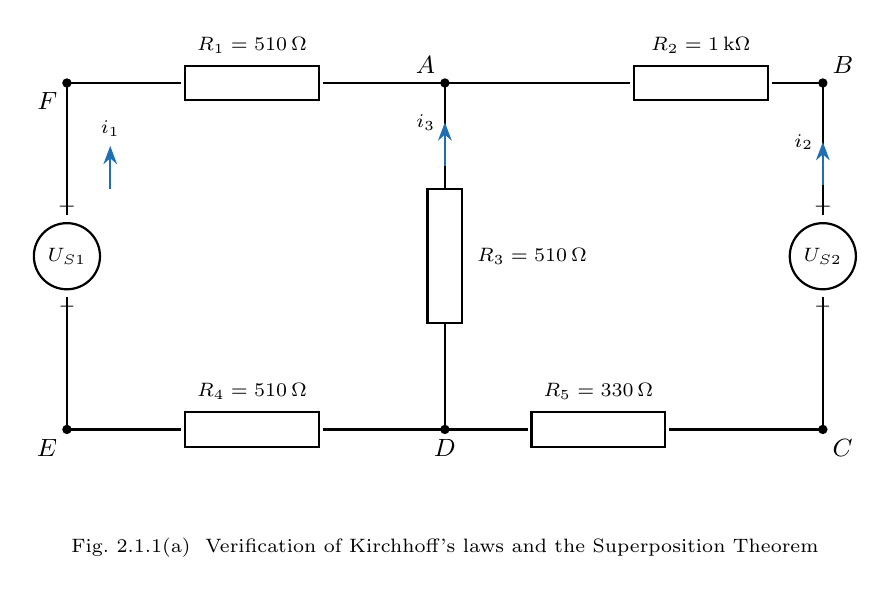
\begin{tikzpicture}[scale=1.0,>=Stealth]
  \coordinate (F) at (0,4.4); \coordinate (A) at (4.8,4.4); \coordinate (B) at (9.6,4.4);
  \coordinate (E) at (0,0);   \coordinate (D) at (4.8,0);   \coordinate (C) at (9.6,0);
  \draw[thick] (F) -- (1.45,4.4); \draw[thick] (3.25,4.4) -- (A);
  \draw[thick] (A) -- (7.15,4.4); \draw[thick] (8.95,4.4) -- (B);
  \resh{2.35}{4.4}{$R_1=510\,\Omega$}
  \resh{8.05}{4.4}{$R_2=1\,\mathrm{k}\Omega$}
  \draw[thick] (E) -- (1.45,0); \draw[thick] (3.25,0) -- (D);
  \draw[thick] (D) -- (5.85,0); \draw[thick] (7.65,0) -- (C);
  \resh{2.35}{0}{$R_4=510\,\Omega$}
  \resh{6.75}{0}{$R_5=330\,\Omega$}
  \draw[thick] (A) -- (4.8,3.05); \draw[thick] (4.8,1.35) -- (D);
  \resv{4.8}{2.2}{$R_3=510\,\Omega$}
  \draw[thick] (E) -- (0,1.68); \draw[thick] (0,2.72) -- (F);
  \draw[thick] (B) -- (9.6,2.72); \draw[thick] (9.6,1.68) -- (C);
  \src{0}{2.2}{$U_{S1}$}
  \src{9.6}{2.2}{$U_{S2}$}
  \fill (F) circle (1.7pt); \node[below left]  at (F) {\small $F$};
  \fill (A) circle (1.7pt); \node[above left]  at (A) {\small $A$};
  \fill (B) circle (1.7pt); \node[above right] at (B) {\small $B$};
  \fill (E) circle (1.7pt); \node[below left]  at (E) {\small $E$};
  \fill (D) circle (1.7pt); \node[below]       at (D) {\small $D$};
  \fill (C) circle (1.7pt); \node[below right] at (C) {\small $C$};
  \draw[->,acc2,thick] (0.55,3.05) -- (0.55,3.6); \node[above] at (0.55,3.6) {\scriptsize $i_1$};
  \draw[->,acc2,thick] (9.6,3.1) -- (9.6,3.65); \node[left] at (9.6,3.65) {\scriptsize $i_2$};
  \draw[->,acc2,thick] (4.8,3.35) -- (4.8,3.9);  \node[left] at (4.8,3.9) {\scriptsize $i_3$};
  \node[below=1.1cm] at (4.8,-0.15) {\scriptsize Fig.~2.1.1(a)\ \ Verification of Kirchhoff's laws and the Superposition Theorem};
\end{tikzpicture}
\end{center}
\en{Draw the six nodes $A,B,C,D,E,F$ as solid dots and label them; draw resistors as rectangles with
their values; draw each source as a circle with its $\pm$ polarity and label $U_{S1},U_{S2}$; mark the
reference directions of $i_1,i_2,i_3$ as shown. The node letters must match the quantities
$U_{AB},U_{CD},U_{AD},U_{DE},U_{FA}$ in the tables.}
\zh{六个节点 $A,B,C,D,E,F$ 画实心点并标注；电阻画矩形、旁边写阻值；电源画圆并标 $\pm$ 极与 $U_{S1},U_{S2}$；
三个电流参考方向 $i_1,i_2,i_3$ 按图。节点字母必须与表中 $U_{AB},U_{CD},U_{AD},U_{DE},U_{FA}$ 对应。}

\section{Table 2.1.2\quad Resistance measurement（电阻测量）}
\begin{center}
\small\setlength{\tabcolsep}{5pt}
\begin{tabular}{@{}l*{7}{c}@{}}
\toprule
Resistor & $R_1$ & $R_2$ & $R_3$ & $R_4$ & $R_5$ & $R_0$ & $R_L$\\
\midrule
Nominal value $/\Omega$ & 510 & 1000 & 510 & 510 & 330 & 51 & 220\\
Measured value $/\Omega$ & 504.2 & 986.6 & 503.4 & 503.9 & 326.1 & 51.3 & 216.4\\
Relative error $/\%$ & 1.14 & 1.34 & 1.29 & 1.20 & 1.18 & 0.59 & 1.64\\
\bottomrule
\end{tabular}
\end{center}
\en{Worked example (to be written next to the table):
$\delta_{R_2}=\dfrac{|986.6-1000|}{1000}\times100\%=1.34\%$. The other resistors are treated in the
same way ($R_1$: $5.8/510=1.14\%$; $R_5$: $3.9/330=1.18\%$). All relative errors are below $2\%$,
so the components are accurate and the measured values can be used directly in the following
calculations.}
\zh{过程写法（表旁）：$\delta_{R_2}=|986.6-1000|/1000\times100\%=1.34\%$。其余同法（$R_1$：$5.8/510=1.14\%$；
$R_5$：$3.9/330=1.18\%$）。全部误差 $<2\%$，精度良好，后续计算直接采用实测值。}

\section{Table 2.1.3\quad Verification of Kirchhoff's laws（基尔霍夫定律验证）}
\en{Experimental conditions: $U_{S1}=6$~V, $U_{S2}=12$~V (the measured source voltages are 5.9~V and
12.1~V and are entered in the table).}
\zh{实验条件 $U_{S1}=6$~V、$U_{S2}=12$~V，电源实测 5.9~V、12.1~V，填入表内。}

\begin{center}
\scriptsize\setlength{\tabcolsep}{3.0pt}
\begin{tabular}{@{}l*{10}{c}@{}}
\toprule
Quantities & $U_{S1}$/V & $U_{S2}$/V & $I_1$/mA & $I_2$/mA & $I_3$/mA & $U_{AB}$/V & $U_{CD}$/V & $U_{AD}$/V & $U_{DE}$/V & $U_{FA}$/V\\
\midrule
Measured & 5.9 & 12.1 & 1.8 & 6.0 & 7.9 & -6.0 & -1.9 & 4.0 & 0.9 & 0.9\\
Calculated & 5.9 & 12.1 & 1.86 & 6.15 & 8.00 & -6.07 & -2.00 & 4.03 & 0.94 & 0.94\\
Relative error $/\%$ & 1.7 & 0.8 & 3.0 & 2.4 & 1.3 & 1.1 & 5.2 & 0.7 & 3.8 & 3.8\\
\bottomrule
\end{tabular}
\end{center}
\en{\footnotesize Row labels: Measured 实测值 / Calculated 计算值 / Relative error 相对误差.
Reference directions: $I_2$ from $B$ to $A$, $I_3$ from $A$ to $D$ (as marked in the figure), so
$I_2>0$ means the current actually flows from $B$ to $A$.}
\zh{\footnotesize 行名：Measured 实测值、Calculated 计算值、Relative error 相对误差。
方向：$I_2$ 正方向 $B\to A$，$I_3$ 正方向 $A\to D$；$I_2>0$ 表示实际由 $B$ 流向 $A$。}

\subsection*{How the calculated values are obtained}
\en{With node $D$ as the reference and the measured resistances substituted, the nodal equations give}
\zh{取 $D$ 为参考点，代入实测电阻解节点方程得}
\[
V_A=4.029\ \text{V},\quad V_B=10.095\ \text{V},\quad V_E=-0.935\ \text{V},\quad
V_F=V_E+U_{S1}=4.965\ \text{V}
\]
\en{hence}
\begin{align*}
I_1&=\frac{V_F-V_A}{R_1}=\frac{4.965-4.029}{504.2}\times10^3=1.86\ \text{mA}\\
I_2&=\frac{V_B-V_A}{R_2}=\frac{10.095-4.029}{986.6}\times10^3=6.15\ \text{mA}\\
I_3&=\frac{V_A-V_D}{R_3}=\frac{4.029}{503.4}\times10^3=8.00\ \text{mA}
\end{align*}
\[
U_{AB}=-6.07\ \text{V},\quad U_{CD}=-2.00\ \text{V},\quad U_{AD}=4.03\ \text{V},\quad
U_{DE}=0.94\ \text{V},\quad U_{FA}=0.94\ \text{V}
\]
\zh{由 $I=(V-V')/R$ 换算：$I_1=(V_F-V_A)/R_1$、$I_2=(V_B-V_A)/R_2$、$I_3=V_A/R_3$；
电压直接取节点电位差。}

\subsection*{KVL verification（KVL 验证）}
\en{Loop 1 ($F\to A\to D\to E\to F$):}
\[
U_{FA}+U_{AD}+U_{DE}-U_{S1}=0.9+4.0+0.9-5.9=-0.10\ \text{V}
\]
\en{Loop 2 ($A\to B\to C\to D\to A$), with $U_{BC}$ equal to the source $U_{S2}$ ($B\to C$ positive):}
\[
U_{AB}+U_{BC}+U_{CD}+U_{DA}=-6.0+12.1+-1.9-4.0=0.20\ \text{V}
\]
\en{Both residuals are $\le0.2$~V (relative residual $<3.4\%$), so \ok{KVL is verified}.}
\zh{两条回路的残差均 $\le0.2$~V（相对残差 $<3.4\%$），\ok{KVL 成立}。}

\subsection*{KCL verification（KCL 验证，node $A$）}
\en{At node $A$ the current $I_1$ enters from $F$, $I_2$ enters from $B$ and $I_3$ leaves towards $D$:}
\[
I_1+I_2-I_3=1.8+6.0-7.9=-0.1\ \text{mA},
\qquad \frac{|-0.1|}{7.9}\times100\%=1.3\%
\]
\en{The residual is much smaller than the branch currents, so \ok{KCL is verified}.}
\zh{残差远小于各支路电流，\ok{KCL 成立}。（若要求换节点，可用 $D$：$I_3+U_{DC}/R_5=U_{DE}/R_4$，同样闭合。）}

\section{Table 2.1.4\quad Verification of the Superposition Theorem（叠加定理验证）}
\en{Experimental conditions: $U_{S1}=12$~V, $U_{S2}=6$~V.}
\zh{实验条件 $U_{S1}=12$~V、$U_{S2}=6$~V。}
\begin{center}
\scriptsize\setlength{\tabcolsep}{2.8pt}
\begin{tabular}{@{}l*{10}{c}@{}}
\toprule
Case & $U_{S1}$/V & $U_{S2}$/V & $I_1$/mA & $I_2$/mA & $I_3$/mA & $U_{AB}$/V & $U_{CD}$/V & $U_{AD}$/V & $U_{DE}$/V & $U_{FA}$/V\\
\midrule
$U_{S1}$ acting alone & 12.0 & 0.0 & 8.6 & -2.4 & 6.2 & 2.9 & 0.7 & 3.2 & 4.3 & 4.3 \\
$U_{S2}$ acting alone & 0.0 & 6.0 & -1.2 & 3.6 & 2.4 & -3.6 & -1.1 & 1.2 & -0.6 & -0.6 \\
Both acting & 12.0 & 6.0 & 7.4 & 1.2 & 8.6 & -1.2 & -0.4 & 4.4 & 3.7 & 3.7 \\
$2U_{S2}$ (homogeneity) & 0.0 & 12.0 & -2.4 & 7.2 & 4.8 & -7.2 & -2.4 & 2.4 & -1.2 & -1.2 \\
\bottomrule
\end{tabular}
\end{center}
\en{\footnotesize Case labels: $U_{S1}$ acting alone / $U_{S2}$ acting alone / Both acting /
$2U_{S2}$ (homogeneity check) —— 单独作用 / 共同作用 / 齐次性检验.}
\zh{\footnotesize 工况：单独作用、共同作用、$2U_{S2}$（齐次性）。}

\subsection*{(1) Additivity（可加性）}
\en{Subtracting row 3 from (row 1 + row 2) column by column gives the residuals below.}
\zh{前两行之和与第三行逐列相减，残差如下。}
\begin{center}
\scriptsize\setlength{\tabcolsep}{4pt}
\begin{tabular}{@{}l*{8}{c}@{}}
\toprule
 & $I_1$ & $I_2$ & $I_3$ & $U_{AB}$ & $U_{CD}$ & $U_{AD}$ & $U_{DE}$ & $U_{FA}$\\
\midrule
Residual & 0.0 & 0.0 & 0.0 & 0.5 & 0.0 & 0.0 & 0.0 & 0.0\\
\bottomrule
\end{tabular}
\end{center}
\en{Except for $U_{AB}$, where the difference is 0.5~V, every column has $|\text{residual}|\le0.05$, so
\ok{additivity is verified}. The $U_{AB}$ deviation comes from the reading taken when $U_{S1}$ acted
alone: 2.9~V was recorded, whereas circuit theory with the measured resistances gives 2.39~V,
i.e. an over-reading of 0.5~V.}
\zh{除 $U_{AB}$ 一列相差 0.5~V 外，其余各列 $|$残差$|\le0.05$，\ok{可加性成立}。
$U_{AB}$ 的偏差出在“$U_{S1}$ 单独作用”那一次读数：实测 2.9~V，按实测电阻正演应为 2.39~V，偏高 0.5~V。}

\subsection*{(2) Homogeneity（齐次性）}
\begin{center}
\scriptsize\setlength{\tabcolsep}{4pt}
\begin{tabular}{@{}l*{8}{c}@{}}
\toprule
 & $I_1$ & $I_2$ & $I_3$ & $U_{AB}$ & $U_{CD}$ & $U_{AD}$ & $U_{DE}$ & $U_{FA}$\\
\midrule
Residual & 0.0 & 0.0 & 0.0 & 0.0 & 0.2 & 0.0 & 0.0 & 0.0\\
\bottomrule
\end{tabular}
\end{center}
\en{For $I_1$, $2\times(-1.2\ \text{mA})=-2.4\ \text{mA}$, exactly the measured value of row 4; every
column has a residual $\le0.2$ (only $U_{CD}$ differs by 0.2~V), so \ok{homogeneity is verified}.}
\zh{以 $I_1$ 为例：$2\times(-1.2\,\text{mA})=-2.4\,\text{mA}$，与第四行实测完全一致；各列残差 $\le0.2$（仅 $U_{CD}$ 差 0.2~V），
\ok{齐次性成立}。}

\subsection*{(3) Comparison with theory（与理论值对照）}
\en{Values obtained from the nodal model with the measured resistances, useful for judging the data
quality:}
\zh{用实测电阻正演得到的理论值，用于判断数据质量：}
\begin{center}
\scriptsize\setlength{\tabcolsep}{3.6pt}
\begin{tabular}{@{}l*{8}{c}@{}}
\toprule
Case & $I_1$/mA & $I_2$/mA & $I_3$/mA & $U_{AB}$/V & $U_{CD}$/V & $U_{AD}$/V & $U_{DE}$/V & $U_{FA}$/V\\
\midrule
$U_{S1}$ alone & 8.75 & -2.42 & 6.32 & 2.39 & 0.79 & 3.18 & 4.41 & 4.41 \\
$U_{S2}$ alone & -1.21 & 3.64 & 2.43 & -3.59 & -1.19 & 1.22 & -0.61 & -0.61 \\
Both & 7.53 & 1.22 & 8.75 & -1.20 & -0.40 & 4.40 & 3.80 & 3.80 \\
$2U_{S2}$ & -2.42 & 7.28 & 4.86 & -7.18 & -2.37 & 2.44 & -1.22 & -1.22 \\
\bottomrule
\end{tabular}
\end{center}

\section{$R_3$ replaced by a 1N4007 diode（二极管替换 $R_3$）}
\begin{center}
\small
\begin{tabular}{@{}ccc l@{}}
\toprule
$U_{S1}$/V & $U_{S2}$/V & $I_3$/mA & Case\\
\midrule
12.0 & 0    & 7.8    & $U_{S1}$ acting alone\\
0    & 6.0  & $-1.3$ & $U_{S2}$ acting alone\\
12.0 & 6.0  & 1.5    & both acting\\
0    & 12.0 & $-2.8$ & $U_{S2}$ doubled (homogeneity)\\
\bottomrule
\end{tabular}
\end{center}
\en{\textbf{No}, the Superposition Theorem does not hold. $7.8+(-1.3)=6.5\ \text{mA}\neq1.5\ \text{mA}$,
a difference of 5.0~mA (3.3 times the measured value). A diode is a \textbf{nonlinear element}: its
volt-ampere characteristic is exponential, so neither homogeneity nor additivity applies, while
linearity is the very premise of the theorem. \warn{The theorem is valid only for linear circuits.}
(Note: $2\times(-1.3)=-2.6$ is close to $-2.8$ only because the diode is nearly linear near this
operating point; this coincidence does not mean that homogeneity holds.)}
\zh{\textbf{不成立}。$7.8+(-1.3)=6.5\neq1.5$~mA，差 5.0~mA（为实测值的 3.3 倍）。二极管是\textbf{非线性元件}，
伏安特性为指数关系，既不满足齐次性也不满足可加性，而叠加定理的前提正是电路线性。\warn{叠加定理只适用于线性电路。}
（$2\times(-1.3)=-2.6$ 与 $-2.8$ 接近，只是该工作点附近近似线性的巧合，不能据此认为齐次性成立。）}

\section{Verification of equivalent-transformation conditions（等效变换，第 3--4 页第 3 节）}
\subsection*{Principle（原理）}
\en{A voltage source $U_S$ in series with $R_0$ is equivalent to a current source $I_S$ in parallel
with the same $R_0$, provided}
\zh{电压源 $U_S$ 与 $R_0$ 串联，对外等效于电流源 $I_S$ 与同一 $R_0$ 并联，条件是}
\begin{equation}
\boxed{\,I_S=\frac{U_S}{R_0}\,}\qquad\text{or }U_S=I_SR_0
\end{equation}
\en{Criterion: with the same load $R_L$ connected, the two circuits must give the \textbf{same terminal
voltage $U$ and the same terminal current $I$}.}
\zh{判据：接同一负载 $R_L$ 时，两者的\textbf{端电压 $U$ 与端电流 $I$ 必须完全相同}。}

\begin{center}
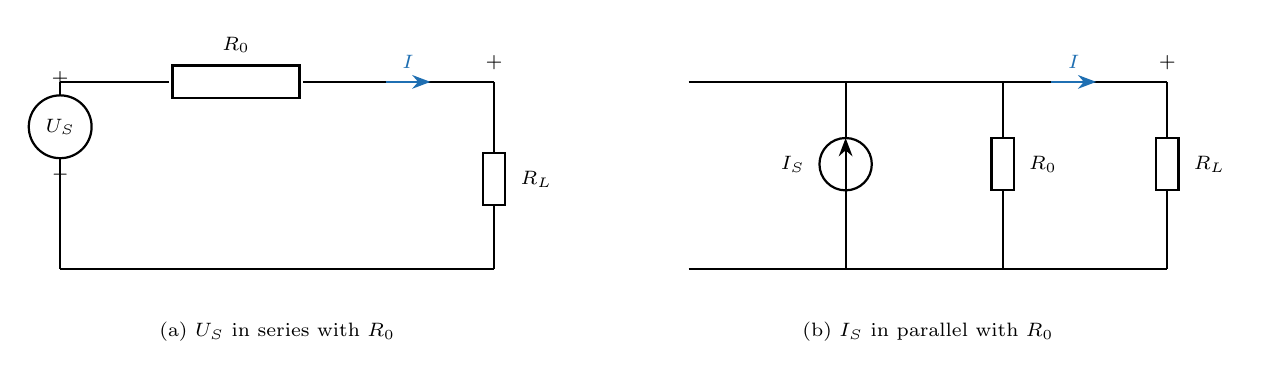
\begin{tikzpicture}[scale=0.95,>=Stealth]
\begin{scope}
  \draw[thick] (0,2.8) -- (0,2.62); \draw[thick] (0,1.78) -- (0,0.3);
  \draw[thick] (0,2.8) -- (1.45,2.8); \draw[thick] (3.25,2.8) -- (4.7,2.8);
  \draw[thick] (4.7,2.8) -- (5.8,2.8); \draw[thick] (5.8,2.8) -- (5.8,1.85);
  \draw[thick] (5.8,1.15) -- (5.8,0.3); \draw[thick] (0,0.3) -- (5.8,0.3);
  \src{0}{2.2}{$U_S$}
  \resh{2.35}{2.8}{$R_0$}
  \draw[fill=white,thick] (5.65,1.15) rectangle (5.95,1.85); \node[right=2pt] at (5.95,1.5) {\scriptsize $R_L$};
  \draw[->,acc2,thick] (4.35,2.8) -- (4.95,2.8) node[midway,above=1pt]{\scriptsize $I$};
  \node[above=1pt] at (5.8,2.8) {\scriptsize $+$};
  \node[below=0.55cm] at (2.9,0.3) {\scriptsize (a) $U_S$ in series with $R_0$};
\end{scope}
\begin{scope}[xshift=8.4cm]
  \draw[thick] (0,2.8) -- (6.4,2.8); \draw[thick] (0,0.3) -- (6.4,0.3);
  \draw[thick] (2.1,2.8) -- (2.1,2.05); \draw[thick] (2.1,1.35) -- (2.1,0.3);
  \draw[thick,fill=white] (2.1,1.7) circle (0.35); \draw[thick,->] (2.1,1.35) -- (2.1,2.05);
  \node[left=1pt] at (1.72,1.7) {\scriptsize $I_S$};
  \draw[thick] (4.2,2.8) -- (4.2,2.05); \draw[thick] (4.2,1.35) -- (4.2,0.3);
  \draw[fill=white,thick] (4.05,1.35) rectangle (4.35,2.05); \node[right=2pt] at (4.35,1.7) {\scriptsize $R_0$};
  \draw[thick] (6.4,2.8) -- (6.4,2.05); \draw[thick] (6.4,1.35) -- (6.4,0.3);
  \draw[fill=white,thick] (6.25,1.35) rectangle (6.55,2.05); \node[right=2pt] at (6.55,1.7) {\scriptsize $R_L$};
  \draw[->,acc2,thick] (4.85,2.8) -- (5.45,2.8) node[midway,above=1pt]{\scriptsize $I$};
  \node[above=1pt] at (6.4,2.8) {\scriptsize $+$};
  \node[below=0.55cm] at (3.2,0.3) {\scriptsize (b) $I_S$ in parallel with $R_0$};
\end{scope}
\end{tikzpicture}
\end{center}

\en{Data and calculations:}
\zh{数据与计算：}
\begin{center}
\footnotesize\setlength{\tabcolsep}{5pt}
\begin{tabular}{@{}lccc c@{}}
\toprule
Circuit & Source value & $U$/V & $I$/mA & $U/I$ /$\Omega$\\
\midrule
(a) $U_S$ in series with $R_0$ & $U_S=6.0$~V & 4.1 & 19.2 & 213.5\\
(b) $I_S$ in parallel with $R_0$ & $I_S=103.5$~mA & 4.1 & 19.2 & 213.5\\
\bottomrule
\end{tabular}
\end{center}

\en{(1) \textbf{External equivalence}: the two connections give exactly the same terminal voltage and
current (4.1~V, 19.2~mA); the port resistance $U/I=213.5\,\Omega$ differs from the load
$R_L=216.4\,\Omega$ by only 1.3~\%, so \ok{the two sources are equivalent to the external circuit}.
(2) \textbf{Check of $I_S=U_S/R_0$}: $I_S^{\text{theo}}=6.0/51.3=117.0$~mA against 103.5~mA measured,
and $U_S^{\text{theo}}=I_SR_0=103.5\times51.3\times10^{-3}=5.31$~V against 6.0~V; the 12~\% difference
comes from the internal resistance of the source, the meters and the leads — the measured 19.2~mA in
circuit (a) implies a total loop resistance of $6.0/19.2\,\text{mA}=312\,\Omega$, about
45~$\Omega$ more than $R_0+R_L=267.7\,\Omega$.
(3) \textbf{Theoretical check of (b)}: $I_L=I_SR_0/(R_0+R_L)=103.5\times51.3/267.7=19.83$~mA
(measured 19.2~mA) and $U_L=19.83\,\text{mA}\times216.4\,\Omega=4.29$~V (measured 4.1~V).}
\zh{(1) \textbf{对外等效}：两种接法的端电压、端电流完全相同（4.1~V、19.2~mA），端口电阻 $U/I=213.5\,\Omega$
与负载 $R_L=216.4\,\Omega$ 只差 1.3\%，故\ok{两个电源对外电路等效}。
(2) \textbf{检验 $I_S=U_S/R_0$}：理论 $I_S=6.0/51.3=117.0$~mA，实测 103.5~mA；理论 $U_S=I_SR_0=5.31$~V，设定 6.0~V。
相差约 12\%，来自电源内阻、表内阻与引线电阻：由图一实测电流反推回路总电阻 $6.0/19.2\,\text{mA}=312\,\Omega$，
比 $R_0+R_L=267.7\,\Omega$ 多出约 45~$\Omega$。
(3) \textbf{图二理论校验}：$I_L=I_SR_0/(R_0+R_L)=19.83$~mA（实测 19.2~mA），$U_L=4.29$~V（实测 4.1~V）。}

\section{Discussion of Results（讨论，第 5 页）}

\subsection*{1. Relative errors from Table 2.1.3}
\en{Filling the third row of Table 2.1.3: \cw{$1.7,\ 0.8,\ 3.0,\ 2.4,\ 1.3,\ 1.1,\ 5.2,\ 0.7,\ 3.8,\ 3.8$} (\%).
All values are below $6\%$; the largest is that of $U_{CD}$ (5.2~\%), simply because its magnitude is
only about 2~V, so the same absolute error gives a larger percentage.}
\zh{填入表 2.1.3 第三行：\cw{$1.7,\ 0.8,\ 3.0,\ 2.4,\ 1.3,\ 1.1,\ 5.2,\ 0.7,\ 3.8,\ 3.8$}（\%）。
全部 $<6\%$；最大是 $U_{CD}$ 的 5.2\%，因其绝对值仅约 2~V，同样绝对误差占比更大。}

\subsection*{2. Verification of KCL at one node}
\en{Take node $A$: $I_1+I_2-I_3=1.8+6.0-7.9=-0.1$~mA, a residual of only 1.3~\%, so KCL is satisfied.
Node $B$ gives the same conclusion: the current through $R_5$ obtained from the voltage is
$U_{CD}/R_5=-1.9/326.1\times10^3=-5.8$~mA, against $I_2=6.0$~mA, a difference of 0.2~mA (3~\%).}
\zh{选节点 $A$：$I_1+I_2-I_3=1.8+6.0-7.9=-0.1$~mA，相对残差 1.3\%，KCL 成立。
选节点 $B$ 同理：由电压换算 $I_{R5}=U_{CD}/R_5=-5.8$~mA，与 $I_2=6.0$~mA 相差 0.2~mA（3\%）。}

\subsection*{3. Superposition and homogeneity from Table 2.1.4}
\en{Take $I_3$, $U_{AD}$ and $I_1$: $6.2+2.4=8.6$~mA; $3.2+1.2=4.4$~V; $2\times(-1.2)=-2.4$~mA, so both
additivity and homogeneity are satisfied. The only exception is $U_{AB}$: $2.9+(-3.6)=-0.7$~V against
$-1.2$~V measured, a 0.5~V difference caused by an over-reading in the first case (theory: 2.39~V).}
\zh{取 $I_3$、$U_{AD}$、$I_1$：$6.2+2.4=8.6$~mA、$3.2+1.2=4.4$~V、$2\times(-1.2)=-2.4$~mA，可加性与齐次性均成立。
唯一例外 $U_{AB}$：$2.9+(-3.6)=-0.7$~V 而实测 $-1.2$~V，差 0.5~V，由第 1 行读数偏高造成（理论 2.39~V）。}

\subsection*{4. Can the power of a resistor be computed by superposition?}
\en{\warn{No.} Power is a quadratic function of current, $P=I^2R$, and does not obey additivity.
For $R_3=503.4\,\Omega$:}
\zh{\warn{不能}。功率是电流的二次函数 $P=I^2R$，不满足可加性。以 $R_3=503.4\,\Omega$ 为例：}
\begin{align*}
P_1&=(6.2\times10^{-3})^2\times503.4=19.4\ \text{mW}\\
P_2&=(2.4\times10^{-3})^2\times503.4=2.9\ \text{mW}\\
P_1+P_2&=22.3\ \text{mW}\quad\text{whereas with both sources}\quad
P=(8.6\times10^{-3})^2\times503.4=37.2\ \text{mW}
\end{align*}
\en{The two results differ by $67\%$. The correct procedure is to \textbf{superpose the currents
first} and then to calculate the power from $P=I^2R$.}
\zh{两者相差 $67\%$。正确做法：\textbf{先叠加电流}得总电流，再按 $P=I^2R$ 求功率。}

\subsection*{5. Does the Superposition Theorem still hold after replacing $R_3$ with a diode?}
\en{\warn{No.} $7.8+(-1.3)=6.5\ \text{mA}\neq1.5\ \text{mA}$. The diode is a nonlinear element whose
volt-ampere characteristic is exponential, so neither additivity nor homogeneity holds, while
linearity is the premise of the theorem. \key{The Superposition Theorem applies only to linear circuits.}}
\zh{\warn{不成立}。$7.8+(-1.3)=6.5$~mA $\neq1.5$~mA。二极管为非线性元件，伏安特性为指数关系，既不满足齐次性也不满足可加性，
而叠加定理的前提正是电路线性。\key{叠加定理只适用于线性电路}。}

\newpage
% ==================== 实验三 ====================
\part*{\centering\color{acc} Experiment 3\quad AC Circuit Experiment\\[0.15cm]
\normalsize 实验三\quad 交流电路实验（实验册第 6--8 页）}
\addcontentsline{toc}{part}{Experiment 3\ \ 实验三（第 6--8 页）}
\markboth{Experiment 3}{Experiment 3}

\section{Preliminary Work（预习作业，第 6 页）}

\subsection*{1. In a parallel AC circuit, can a branch current be larger than the total current?}
\en{\textbf{Yes.} In an AC circuit the currents are \textbf{phasors}, and the total current is the phasor
sum of the branch currents, not their algebraic sum. When the branch currents have different phase
angles (capacitive current leading, inductive current lagging) they partly cancel, so the total current
can be smaller than a single branch current. In this experiment the lamp branch carries about 307~mA
while the total current falls to 143.7~mA.}
\zh{\textbf{能。}交流电流是\textbf{相量}，总电流是各支路电流的相量和而非代数和。各支路相位不同时相互抵消，
总电流可以小于某条支路电流。本实验灯管支路约 307~mA，而总电流最低降到 143.7~mA。}

\subsection*{2. What kind of values are displayed by AC voltmeters and ammeters? Can they be summed algebraically?}
\en{They display \textbf{RMS (effective) values}. These cannot be added algebraically: the RMS values of
sinusoids of different phase do not obey a simple algebraic sum and must be combined as
\textbf{phasors}. For a series $R$--$C$ circuit, $U=\sqrt{U_R^2+U_C^2}$, not $U_R+U_C$.}
\zh{显示\textbf{有效值}。不能代数相加：不同相位正弦量的有效值不满足代数关系，必须按\textbf{相量}合成。
串联 $R$-$C$ 电路有 $U=\sqrt{U_R^2+U_C^2}$，而不是 $U_R+U_C$。}

\subsection*{3. Should the voltage-coil external connection or the current-coil external connection be used when measuring active power?}
\en{It \textbf{depends on the load impedance}; the aim is to make the power consumed by the wattmeter
itself negligible. For a \textbf{small load impedance} (large load current) the voltage coil should be
connected on the supply side (voltage-coil first), so that the voltage drop of the current coil is
negligible. For a \textbf{large load impedance} (small load current) the voltage coil should be
connected on the load side, so that the current taken by the voltage coil is negligible.}
\zh{\textbf{取决于负载阻抗}，原则是让功率表自身损耗对读数影响最小。负载阻抗\textbf{较小}（负载电流大）时用
\textbf{电压线圈前接}（接在电源侧），电流线圈压降影响可忽略；负载阻抗\textbf{较大}（负载电流小）时用
\textbf{电压线圈后接}（接在负载侧），电压支路分流影响可忽略。}

\subsection*{4. Phasor diagram: how does a small capacitor in parallel identify the nature of the load?}
\en{Take the terminal voltage as the reference phasor; the capacitive current leads it by $90^\circ$.
Adding the capacitive current to the load current moves the resultant \textbf{closer} to the voltage
when the load is \textbf{inductive} (total current decreases), \textbf{further away} when the load is
\textbf{capacitive} (total current increases), and leaves it almost unchanged when the load is
\textbf{resistive}. Here the total current first decreases and then increases, with a minimum near
$C=3.7\,\mu$F, so the lamp with its ballast is an \textbf{inductive load}.}
\zh{以端电压为参考相量，容性电流超前 $90^\circ$。与负载电流相加后：感性负载时合成电流\textbf{更靠近}电压、总电流减小；
容性负载时\textbf{更远离}、总电流增大；阻性负载时基本不变。本实验总电流先减后增、最小值在 $C=3.7\,\mu$F 附近，
故日光灯（含镇流器）为\textbf{感性负载}。}

\begin{center}
\begin{tikzpicture}[scale=0.95,>=Stealth]
  \draw[->,thick] (0,0) -- (4.6,0) node[right] {\small $\dot U$};
  \draw[->,thick,acc2] (0,0) -- (1.5,-2.9) node[below right] {\small $\dot I_L$};
  \draw[->,thick,okc] (0,0) -- (0,2.4) node[above] {\small $\dot I_C$};
  \draw[->,thick,warnc] (0,0) -- (1.5,-0.5) node[right] {\small $\dot I=\dot I_L+\dot I_C$};
  \draw[dashed,gray] (1.5,-2.9) -- (1.5,0);
  \draw[->,gray] (1.5,2.4) -- (1.5,-2.9);
  \draw (0.6,0) arc (0:-62:0.6);
  \node at (1.05,-0.32) {\scriptsize $\varphi$};
\end{tikzpicture}
\end{center}

\section{Wiring of the fluorescent-lamp circuit（日光灯接线，图 2.3.3）}
\en{\textbf{Connection sequence}: AC supply $\to$ knife switch $\to$ fuse $\to$ current coil of the
wattmeter $\to$ ballast $\to$ lamp $\to$ back to the neutral line. The voltage coil of the wattmeter is
connected across the lamp (or across the supply). The capacitor bank is connected \textbf{in parallel
with the supply}, each capacitor through its own switch.}
\zh{\textbf{接线顺序}：交流电源 $\to$ 闸刀开关 $\to$ 熔断器 $\to$ 功率表电流线圈 $\to$ 镇流器 $\to$ 灯管 $\to$ 回零线；
功率表电压线圈并在灯管（或电源）两端；电容器组经各自开关\textbf{并联在电源两端}。}
\en{\textbf{Safety (must be written in the report)}: after wiring, check the circuit yourself but
\warn{do not switch on the supply yourself}; ask the teacher to inspect and energize the circuit.
Switch off and verify dead before changing any connection.}
\zh{\textbf{必须写进报告的安全要求}：接线后先自查，\warn{不得自行合闸}，须请指导教师检查后由教师送电；改接线路前必须断电验电。}

\section{Fluorescent-lamp data（表 2.3.4 / 2.3.5）}
\en{Measured: $C,U,U_R,U_L,I,I_C,I_L,P,P_{LR},P_C$. To be computed: $\cos\varphi=P/(UI)$ with $I$ in
amperes.}
\zh{实测：$C,U,U_R,U_L,I,I_C,I_L,P,P_{LR},P_C$；需计算：$\cos\varphi=P/(UI)$（$I$ 用安培）。}
\begin{center}
\scriptsize\setlength{\tabcolsep}{2.2pt}
\begin{tabular}{@{}c*{11}{c}@{}}
\toprule
$C/\mu$F & $U$/V & $U_R$/V & $U_L$/V & $I$/mA & $I_C$/mA & $I_L$/mA & $P$/W & $P_{LR}$/W & $P_C$/W & $\cos\varphi$ calc. & $\cos\varphi$ meas.\\
\midrule
0.0 & 219.6 & 194.5 & 56.7 & 313.4 & 0.0 & 307.2 & 28.4 & 28.9 & 0.0 & 0.413 & 0.426 \\
1.0 & 219.6 & 194.5 & 56.7 & 274.8 & 43.2 & 307.9 & 28.4 & 28.9 & 0.0 & 0.471 & 0.485 \\
2.0 & 219.6 & 194.5 & 56.7 & 198.5 & 139.9 & 306.9 & 28.4 & 28.9 & 0.0 & 0.652 & 0.678 \\
3.7 & 219.6 & 194.5 & 56.7 & 143.7 & 304.2 & 306.9 & 28.2 & 28.8 & 0.0 & 0.894 & 0.989 \\
4.7 & 219.6 & 194.5 & 56.7 & 159.9 & 346.9 & 307.5 & 28.2 & 28.9 & 0.0 & 0.803 & 0.904 \\
5.7 & 219.6 & 194.5 & 56.7 & 222.3 & 443.5 & 308.1 & 28.2 & 28.9 & 0.0 & 0.578 & 0.638 \\
\bottomrule
\end{tabular}
\end{center}
\en{\footnotesize Also $P_L=14.1$~W (lamp) and $P_R=14.4$~W (ballast); their sum 28.5~W agrees with the
total power 28.4~W.}
\zh{\footnotesize 另：灯管功率 $P_L=14.1$~W，镇流器功率 $P_R=14.4$~W，二者之和 28.5~W 与总功率 28.4~W 相符。}

\subsection*{Worked examples for the $\cos\varphi$ column}
\en{%
$C=0.0\,\mu\text{F}:\ \cos\varphi=\dfrac{P}{UI}=\dfrac{28.4}{219.6\times0.3134}=0.413$ (measured 0.426, difference 3.1\%);\\
$C=3.7\,\mu\text{F}:\ \cos\varphi=\dfrac{28.2}{219.6\times0.1437}=0.894$ (measured 0.989, difference 9.6\%).}
\zh{计算列示范两行即可，写法同上；计算值与实测趋势一致、量级相符，差异来自功率表与电流表的接入损耗。}

\en{Supplementary quantities for the analysis ($S=UI$, $Q=\sqrt{S^2-P^2}$, $I_C^{\text{theo}}=\omega CU$):}
\zh{分析用补充量（$S=UI$，$Q=\sqrt{S^2-P^2}$，$I_C^{\text{theo}}=\omega CU$）：}
\begin{center}
\scriptsize\setlength{\tabcolsep}{4pt}
\begin{tabular}{@{}cccccc@{}}
\toprule
$C/\mu$F & $S$/VA & $Q$/var & $I_C^{\text{theo}}$/mA & $\cos\varphi$ calc. & Deviation\\
\midrule
0.0 & 68.8 & 62.7 & 0 & 0.413 & 3.1\% \\
1.0 & 60.3 & 53.2 & 69 & 0.471 & 3.0\% \\
2.0 & 43.6 & 33.1 & 138 & 0.652 & 3.9\% \\
3.7 & 31.6 & 14.2 & 255 & 0.894 & 9.6\% \\
4.7 & 35.1 & 20.9 & 324 & 0.803 & 11.2\% \\
5.7 & 48.8 & 39.8 & 393 & 0.578 & 9.5\% \\
\bottomrule
\end{tabular}
\end{center}

\subsection*{Compensation effect（补偿效果分析）}
\en{\begin{itemize}
  \item After the capacitor is connected the branch current $I_L$ stays almost constant (about 307~mA),
        while the total current $I$ falls from 313.4~mA to a minimum of 143.7~mA at $C=3.7\,\mu$F and then
        rises again to 222.3~mA;
  \item the power factor rises from 0.413 to 0.894--0.989, i.e. $\varphi$ falls from $65.6^\circ$ to about $8.5^\circ$;
  \item at the minimum current the reactive power is also a minimum ($Q=14.2$~var), showing that the
        capacitive reactive power exactly compensates the inductive one;
  \item the optimum capacitance is
        $C_{\text{opt}}=\dfrac{P\tan\varphi_0}{\omega U^2}=\dfrac{28.4\times\tan65.6^\circ}{2\pi\times50\times219.6^2}\times10^6=4.14\ \mu\text{F}$,
        in good agreement with the measured minimum at $3.7\,\mu$F.
\end{itemize}}
\zh{\begin{itemize}
  \item 并入电容后灯管支路电流 $I_L$ 基本不变（约 307~mA），总电流 $I$ 由 313.4~mA 降到最低 143.7~mA（$C=3.7\,\mu$F），
        再回升到 222.3~mA；
  \item 功率因数由 0.413 提高到 0.894--0.989，即 $\varphi$ 由 $65.6^\circ$ 降到约 $8.5^\circ$；
  \item 总电流最小时无功功率也最小（$Q=14.2$~var），说明容性无功恰好补偿掉感性无功；
  \item 理论最佳电容 $C_{\text{opt}}=P\tan\varphi_0/(\omega U^2)=4.14\,\mu$F，与实测最小电流对应的 3.7\,$\mu$F 基本一致。
\end{itemize}}

\section{Ignition voltage（点火电压，第 8 页）}
\en{The measured ignition voltage of the fluorescent lamp is \cw{173.3~V}.
A cold lamp needs a voltage higher than its operating voltage to break down the gas; this voltage is
provided by the self-induced e.m.f.\ of the ballast at the instant the starter opens. Once the lamp is
lit the ballast acts as a current limiter and the lamp operates at about 56.7~V and 0.3~A.}
\zh{日光灯点火电压实测 \cw{173.3~V}。灯管冷态需高于工作电压的电压才能击穿气体放电，该电压由镇流器在启辉器断开瞬间
产生的自感电动势提供；点燃后镇流器转为限流作用，灯管工作在约 56.7~V、0.3~A。}

\section{Voltage-triangle relationship（电压三角形，第 8 页第 2 节）}
\en{A capacitor $C$ is connected in series with a resistive load; a voltmeter measures the load voltage
$U_R$, the capacitor voltage $U_C$ and the total voltage $U$.}
\zh{电容 $C$ 与阻性负载串联接在交流电源上，用电压表分别测负载电压 $U_R$、电容电压 $U_C$ 与总电压 $U$。}

\begin{center}
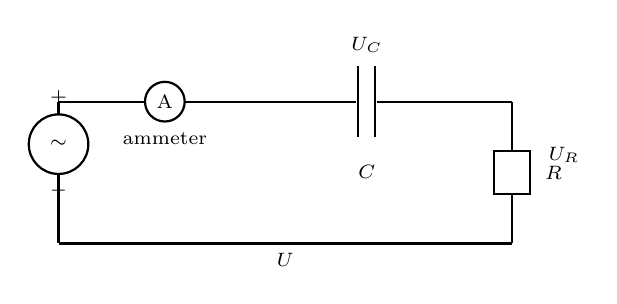
\begin{tikzpicture}[scale=0.9,>=Stealth]
  \draw[thick] (0,2.4) -- (0,2.22); \draw[thick] (0,1.38) -- (0,0.4);
  \draw[thick] (0,2.4) -- (1.5,2.4); \draw[thick] (1.5,2.4) -- (2.6,2.4);
  \draw[thick,fill=white] (1.5,2.4) circle (0.28); \node at (1.5,2.4) {\scriptsize A};
  \draw[thick] (2.6,2.4) -- (4.2,2.4); \draw[thick] (4.5,2.4) -- (4.9,2.4);
  \capsym{4.35}{2.4}{}
  \node[below=0.68cm] at (4.35,2.4) {\scriptsize $C$};
  \node[above] at (4.35,2.95) {\scriptsize $U_C$};
  \draw[thick] (4.9,2.4) -- (6.4,2.4); \draw[thick] (6.4,2.4) -- (6.4,1.7);
  \draw[fill=white,thick] (6.15,1.1) rectangle (6.65,1.7); \node[right=2pt] at (6.65,1.4) {\scriptsize $R$};
  \draw[thick] (6.4,1.1) -- (6.4,0.4); \draw[thick] (6.4,0.4) -- (0,0.4);
  \src{0}{1.8}{$\sim$}
  \node[below] at (1.5,2.1) {\scriptsize ammeter};
  \node[right=2pt] at (6.7,1.65) {\scriptsize $U_R$};
  \node[below] at (3.2,0.4) {\scriptsize $U$};
\end{tikzpicture}
\end{center}

\begin{center}
\small\setlength{\tabcolsep}{7pt}
\begin{tabular}{@{}lccc@{}}
\toprule
 & $C=1\,\mu$F & $C=2\,\mu$F & $C=4.7\,\mu$F\\
\midrule
$U_R$/V (measured) & 219.1 & 218.9 & 215.2\\
$U_C$/V (measured) & 19.9 & 23.3 & 43.8\\
$U$/V (measured) & 220.1 & 220.1 & 220.1\\
$\sqrt{U_R^2+U_C^2}$/V & 220.0 & 220.1 & 219.6\\
Deviation $/\%$ & -0.04 & +0.02 & -0.22\\
$\varphi=\arctan(U_C/U_R)$ & 5.2$^\circ$ & 6.1$^\circ$ & 11.5$^\circ$\\
\bottomrule
\end{tabular}
\end{center}

\en{Worked example (one line is enough in the report):}
\zh{验证过程（报告里写一行示范即可）：}
\par\noindent\quad $C=1\,\mu$F: $\sqrt{U_R^2+U_C^2}=\sqrt{219.1^2+19.9^2}=220.0$~V vs.\ measured $U=220.1$~V, deviation -0.04\%\\
\quad $C=2\,\mu$F: $\sqrt{U_R^2+U_C^2}=\sqrt{218.9^2+23.3^2}=220.1$~V vs.\ measured $U=220.1$~V, deviation +0.02\%\\
\quad $C=4.7\,\mu$F: $\sqrt{U_R^2+U_C^2}=\sqrt{215.2^2+43.8^2}=219.6$~V vs.\ measured $U=220.1$~V, deviation -0.22\%\\
\par
\en{All three deviations are below $0.3\%$, so $U=\sqrt{U_R^2+U_C^2}$ is \ok{verified}: in a series
$R$--$C$ circuit the total voltage is the \textbf{phasor sum} of $U_R$ and $U_C$, and the three form a
right triangle with angle $\varphi$, where $\cos\varphi=U_R/U$.}
\zh{三组偏差均 $<0.3\%$，故 $U=\sqrt{U_R^2+U_C^2}$ \ok{成立}：串联 $R$-$C$ 电路中总电压是 $U_R$ 与 $U_C$ 的\textbf{相量和}，
三者构成以 $\varphi$ 为夹角的直角三角形，且 $\cos\varphi=U_R/U$。}

\section{Conclusions of Experiment 3（实验三结论）}
\en{\begin{enumerate}
  \item Connecting capacitors in parallel compensates the reactive power of an inductive load and raises
        the power factor: $\cos\varphi$ rises from 0.413 to about 0.894 while the total current falls from
        313.4~mA to 143.7~mA, the branch current and the active power remaining almost unchanged.
  \item There is an optimum capacitance (3.7--4.7\,$\mu$F here, 4.14\,$\mu$F theoretically);
        over-compensation makes the total current rise again and the power factor fall
        ($\cos\varphi=0.638$ at $C=5.7\,\mu$F).
  \item In a series $R$--$C$ circuit the voltages satisfy $U=\sqrt{U_R^2+U_C^2}$, which verifies the
        phasor (voltage-triangle) relation for AC quantities.
  \item AC meters indicate RMS values, which cannot be added algebraically but must be combined as phasors.
\end{enumerate}}
\zh{\begin{enumerate}
  \item 并联电容可补偿感性负载无功、提高功率因数：$\cos\varphi$ 由 0.413 提高到约 0.894，总电流由 313.4~mA 降到 143.7~mA，
        而负载支路电流与有功功率几乎不变。
  \item 补偿电容存在最佳值（本实验 3.7--4.7\,$\mu$F，理论 4.14\,$\mu$F）；过补偿会使总电流增大、功率因数下降
        （$C=5.7\,\mu$F 时 0.638）。
  \item 串联 $R$-$C$ 电路满足 $U=\sqrt{U_R^2+U_C^2}$，验证了交流量的相量（三角形）关系。
  \item 交流表读数为有效值，不能代数相加，必须按相量合成。
\end{enumerate}}

\newpage
\appendix
\section{Quick reference: what to write in each cell（速查）}
\begin{center}
\footnotesize\setlength{\tabcolsep}{3pt}
\begin{tabularx}{\linewidth}{@{}p{2.2cm}p{2.3cm}X@{}}
\toprule
Table & Row & Content / 内容\\
\midrule
2.1.2 & Nominal & 510, 1000, 510, 510, 330, 51, 220~$\Omega$\\
 & Measured & 504.2, 986.6, 503.4, 503.9, 326.1, 51.3, 216.4~$\Omega$\\
 & Rel.\ error & 1.14, 1.34, 1.29, 1.20, 1.18, 0.59, 1.64~\%\\
\midrule
2.1.3 & Measured & 5.9, 12.1, 1.8, 6.0, 7.9, $-6.0$, $-1.9$, 4.0, 0.9, 0.9\\
 & Calculated & 6.0, 12.0, 1.86, 6.15, 8.00, -6.07, -2.00, 4.03, 0.94, 0.94\\
 & Rel.\ error & 1.7, 0.8, 3.0, 2.4, 1.3, 1.1, 5.2, 0.7, 3.8, 3.8~\%\\
\midrule
2.1.4 & 4 rows & see the table in the text（见正文）\\
 & checks & two residual tables + one conclusion sentence\\
\midrule
Diode & 4 rows & 7.8, $-1.3$, 1.5, $-2.8$~mA\\
\midrule
Equiv. & 2 rows & (a) 4.1~V / 19.2~mA;\ (b) 4.1~V / 19.2~mA\\
\midrule
Lamp & 6 rows & $\cos\varphi$ calc.: 0.413, 0.471, 0.652, 0.894, 0.803, 0.578\\
\midrule
V-triangle & 6 rows & $\sqrt{U_R^2+U_C^2}$: 220.0, 220.1, 219.6~V; deviations $\le0.22\%$\\
\midrule
Ignition & one cell & 173.3~V\\
\bottomrule
\end{tabularx}
\end{center}

\section{Common mistakes（常见失分点）}
\en{\begin{enumerate}
  \item Writing numbers without formulas: always quote the formula first, e.g.
        $\delta=\frac{|x_{\text{meas}}-x_{\text{calc}}|}{|x_{\text{calc}}|}\times100\%$.
  \item Inconsistent significant figures: 1 decimal for U and I, 1--2 decimals for relative errors.
  \item Wrong reference directions: $I_2$ and $I_3$ must follow the arrows, otherwise KCL contradicts itself.
  \item KVL loop direction: positive when the loop direction agrees with the reference direction, negative otherwise.
  \item Forgetting the scope of the Superposition Theorem: linear circuits only, and only for voltages
        and currents — power cannot be superposed.
  \item Adding AC quantities algebraically: $U=\sqrt{U_R^2+U_C^2}$ must be justified by the phasor diagram.
  \item Omitting the safety statement: the fluorescent-lamp circuit must be energized by the teacher after inspection.
\end{enumerate}}
\zh{\begin{enumerate}
  \item 只写数不写公式；\quad 2. 有效数字混乱；\quad 3. 参考方向与箭头不一致使 KCL 自相矛盾；\quad
  4. KVL 绕行方向符号取错；\quad 5. 忘了叠加定理只适用于线性电路的电压、电流，功率不能叠加；\quad
  6. 交流量代数相加；\quad 7. 漏写“经教师检查后送电”的安全说明。
\end{enumerate}}

\section{Data provenance（数据来源说明）}
\en{All measured data come from the 8 scanned pages of your lab notebook and were checked with you
before being frozen. Calculated values were obtained from the nodal model with
$R_1=504.2$, $R_2=986.6$, $R_3=503.4$, $R_4=503.9$, $R_5=326.1\ \Omega$; their deviations from the
measurements are all below $6\%$, so the recorded data are self-consistent and can be used directly.}
\zh{实测数据取自你的实验记录本扫描件（8 页），并与你逐表核对后冻结；计算值用 $R_1=504.2$、$R_2=986.6$、
$R_3=503.4$、$R_4=503.9$、$R_5=326.1\ \Omega$ 按节点电压法正演得到，与实测偏差均 $<6\%$，说明数据内部自洽，可直接作为报告依据。}

\end{document}
